% 原文 p.106（後半）


\subsubsectionlink{Wigner表示}
Wigner表示、またはWigner関数は、連続自由度で記述される系に対して、密度行列の代わりに、しばしば用いられる。典型的には、この自由度は系の位置$x$であり、ここではその場合に注目する。系の純粋状態または混合状態の、位置空間密度行列$\rho(x,x')\equiv\langle x\rvert\hat\rho\lvert x'\rangle$が与えられたとき、Wigner関数を\cite{ref149,ref150}
\begin{equation}W(x,p)\equiv\frac1{2\pi}\int_{-\infty}^{+\infty}\mathrm dy\,e^{ipy}\rho(x+y/2,x-y/2)\tag{2.132}\end{equation}
と定義する。ここで$p$は粒子の運動量、あるいは一般的に$x$の共役変数である。

Wigner関数は、位相空間の古典的確率分布と、いくらか似ている。たとえば$W(x,p)$は$x$、$p$の実数値関数であり、$x$、$p$の確率分布$P(x)\equiv\rho(x,x)$、$P(p)\equiv\widetilde\rho(p,p)\equiv\langle p\rvert\hat\rho\lvert p\rangle$は、$W(x,p)$の周辺分布として回復できる。
\begin{align}P(x)=\rho(x,x)&=\int\mathrm dp\,W(x,p),\tag{2.133}\\P(p)=\widetilde\rho(p,p)&=\int\mathrm dx\,W(x,p).\tag{2.134}\end{align}
また、$\int\mathrm dx\int\mathrm dp\,W(x,p)=\operatorname{Tr}(\hat\rho)=1$である。

% 原文 p.107
\hypertarget{srcpage:107}{}\label{srcpage:107}
しかし、Wigner関数と位相空間の確率分布を同一視したくなる、この誘惑を行き過ぎさせてはならないことを示す、重要な注意点がある。最も重要なのは、Wigner関数が一般に、ある領域で負の値を取り、真の確率分布を表せないことを示す点である。実際、純粋状態のWigner関数に負の値がないのは、状態がGaussianである場合、かつその場合に限ると示せる\cite{ref151}。もちろん、この知見は、それほど驚くべきでない。結局、量子力学の不確定性関係は、位置と運動量を任意の精度で同時に決定することを禁じる。したがって、端的に言えば、実際の量子的位相空間分布は、そもそも存在できないのである。

このような注意にもかかわらず、多くの場合、Wigner関数は、位相空間の位置と運動量の相関や、量子的干渉を、うまく可視化してくれる。Wigner関数を使って「二重スリット型」の重ね合わせを表し、位相空間のデコヒーレンスの力学を研究することは、Zurek\cite{ref013}に遡る。本書では、5.2節の量子Brown運動の研究に、Wigner関数を用いる。

Wigner関数の姿について感覚を得るため、位置空間で距離$\Delta x$だけ離れた、二つのGaussian波束の重ね合わせを考えよう（図2.7）。対応するWigner関数を図2.8に示す。二つの主ピークと、振動する模様が見える。直接ピークともしばしば呼ばれる主ピークは、古典的に予想される位相空間領域、すなわち位置は$\Delta x$だけ離れ、運動量方向の広がりは同じ領域にある。したがって、これらは、重ね合わされた二つのピークが記述する「古典的」位相空間分布に似たものを記述すると見なせる。位置空間のかなり狭い局在の帰結である、運動量方向の大きな広がりが明瞭に見える。不確定性原理によれば、位置と運動量の両方で完全に局在することはできず、位置の局在がよいほど、運動量方向の広がりは大きい。

\begin{figure}[htbp]\centering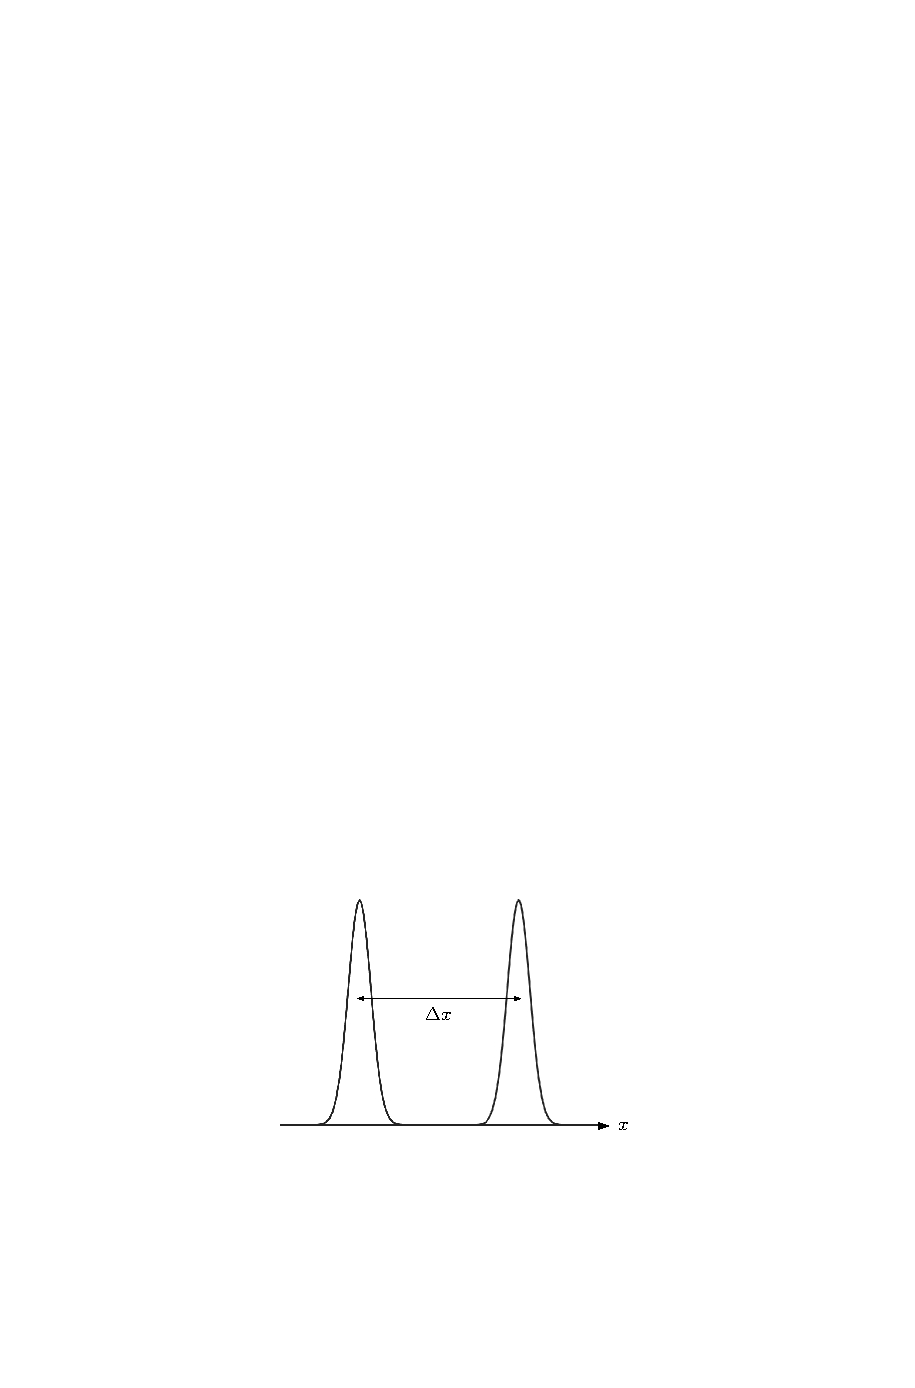
\includegraphics[width=.62\linewidth]{figures/ch02_fig07.pdf}\caption{空間で$\Delta x$だけ離れた、二つのGaussian波束の重ね合わせの図。}\end{figure}

% 原文 p.108
\hypertarget{srcpage:108}{}\label{srcpage:108}
\begin{figure}[htbp]\centering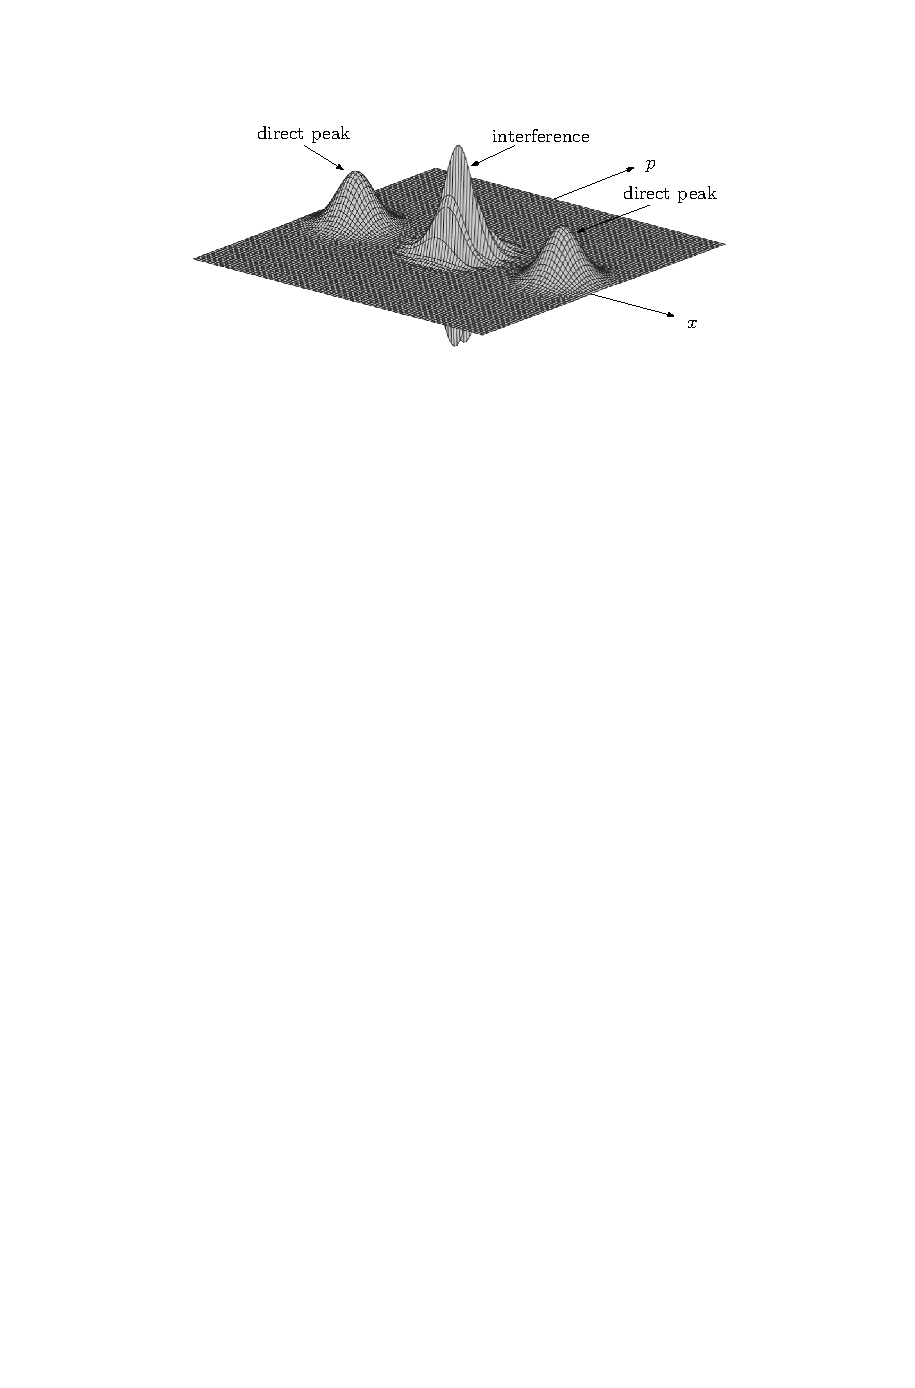
\includegraphics[width=.85\linewidth]{figures/ch02_fig08.pdf}\caption{位置空間で離れた二つのGaussian波束の重ね合わせのWigner表示（図2.7）。}\end{figure}

図2.8に見える、二つの主ピークを結ぶ線に平行な尾根を持つ振動模様は、二波束間の量子干渉が存在する証拠である。系の位置を監視する環境との相互作用が、空間的コヒーレンスを抑制すると、この振動が減衰する（図2.9）。これは、位相空間でデコヒーレンスの作用を可視化する、直観的な方法を与える。

ここで考える、空間的に離れた二つのGaussian波束の重ね合わせでは、Wigner関数の振動模様の振動数$f$が、位置空間の波束間隔$\Delta x$に、
\begin{equation}f=\Delta x/\hbar\tag{2.135}\end{equation}
によって直接関係することを示せる。したがって大まかに言えば、重ね合わせ状態が非古典的になるほど、Wigner関数の振動は速くなる。また図2.8から、特に振動模様の領域で、Wigner関数が負の値を取ることも明瞭に分かる。上で論じたとおり、これは、Wigner関数を古典的な位相空間確率分布と解釈できないことを、直接視覚的に示す。

\begin{figure}[htbp]\centering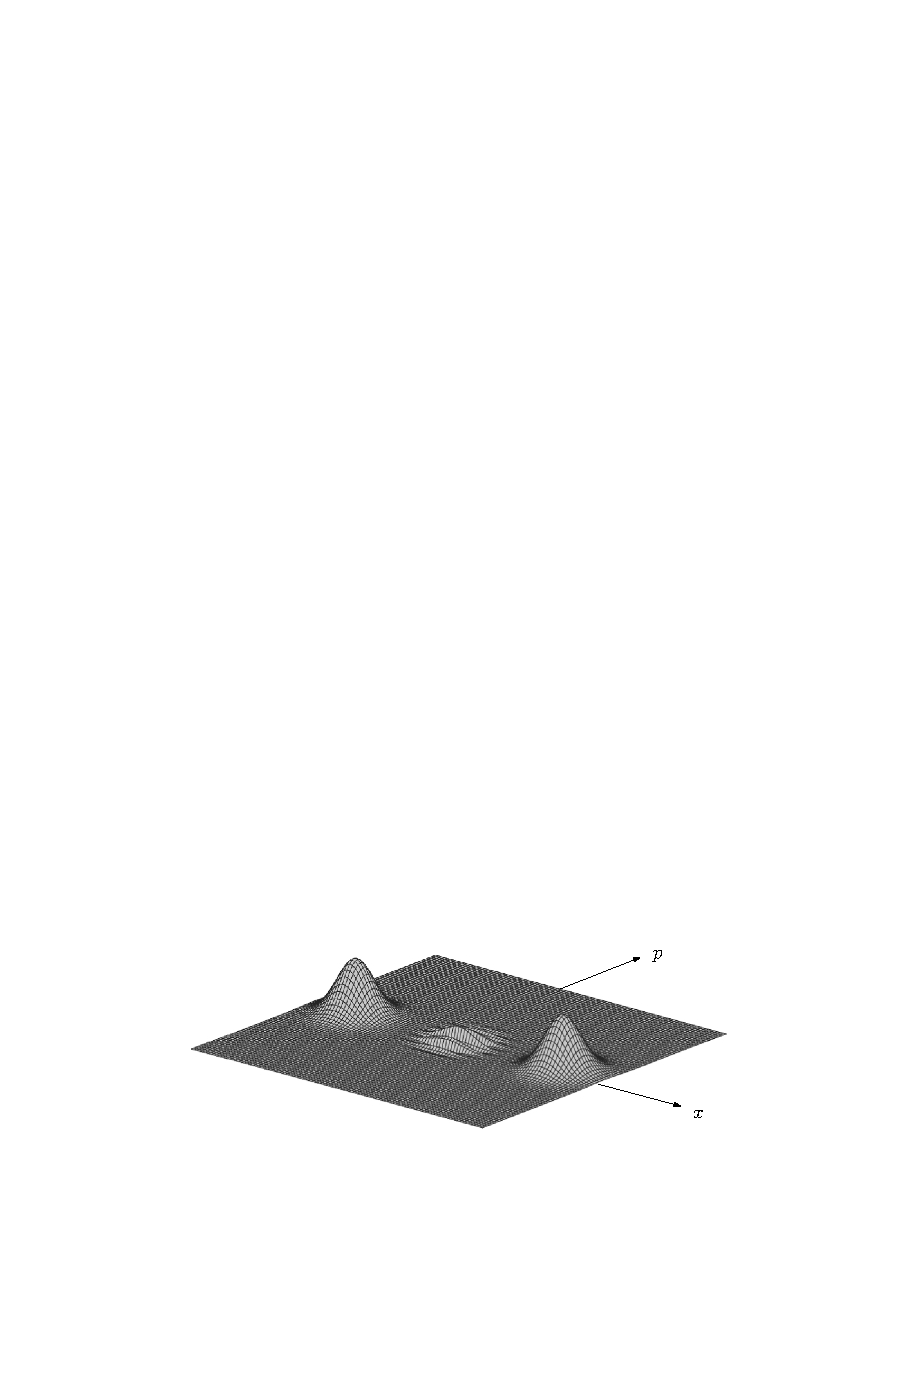
\includegraphics[width=.85\linewidth]{figures/ch02_fig09.pdf}\caption{環境との相互作用と、その結果生じる干渉の抑制は、Wigner表示の振動模様の減衰として現れる（図2.8と比較）。}\end{figure}

% 原文 p.109
\hypertarget{srcpage:109}{}\label{srcpage:109}
\subsubsectionlink{環境の「純粋化」}
2.4.6節でトレース演算を論じた際、より大きな複合系の純粋状態から、部分系の縮約状態を得る方法を示した。私たちの場合、複合系は、関心のある系とその環境である。この手順を「逆にして」、有限次元Hilbert空間で、任意に与えられた非純粋状態を純粋化できることは、驚くべきでない。これは、任意の非純粋状態を、より大きな系の純粋状態の縮約状態と見なせる、という意味である。

証明はまったく直接的である。関心のある系$\mathcal S$が、Hilbert空間$\mathcal H_{\mathcal S}$内の、一般に非純粋な、何らかの密度行列$\hat\rho_{\mathcal S}$で記述されるとする。2.4節、特に式(2.20)から、任意の密度行列は、$\sum_i p_i=1$を満たす非負実数$p_i$を使って、$\hat\rho_{\mathcal S}=\sum_i p_i\lvert\psi_i\rangle\langle\psi_i\rvert$と書ける。「環境」$\mathcal E$と呼んでもよい、別の仮想的な系を導入しよう。もちろん、この第二の系に、特定の物理的役割や表現を結び付ける必要はない。$\mathcal E$のHilbert空間$\mathcal H_{\mathcal E}$を、$\mathcal H_{\mathcal S}$と同じ次元とし、その正規直交基底$\{\lvert\phi_i\rangle\}$を選ぶ。複合系$\mathcal{SE}$の純粋状態を、
\begin{equation}\lvert\Psi\rangle\equiv\sum_i\sqrt{p_i}\lvert\psi_i\rangle\lvert\phi_i\rangle\tag{2.136}\end{equation}
と定義する。その対応する純粋状態の密度行列は、
\begin{equation}\hat\rho=\lvert\Psi\rangle\langle\Psi\rvert=\sum_{ij}\sqrt{p_ip_j}\lvert\psi_i\rangle\langle\psi_j\rvert\otimes\lvert\phi_i\rangle\langle\phi_j\rvert\tag{2.137}\end{equation}
となる。仮想的「環境」$\mathcal E$についてトレースを取れば、単に$\mathcal S$の元の密度行列$\hat\rho_{\mathcal S}$が回復される。
\begin{align}
\operatorname{Tr}_{\mathcal E}\hat\rho&=\sum_k\langle\phi_k\rvert\left[\sum_{ij}\sqrt{p_ip_j}\lvert\psi_i\rangle\langle\psi_j\rvert\otimes\lvert\phi_i\rangle\langle\phi_j\rvert\right]\lvert\phi_k\rangle\tag{2.138}\\
&=\sum_i p_i\lvert\psi_i\rangle\langle\psi_i\rvert=\hat\rho_{\mathcal S}.\tag{2.139}
\end{align}
この「純粋化定理」は、重要な含意を持つ。デコヒーレンスの議論では、一般性を失わずに、関心のある系と相互作用する前に環境は純粋状態にあると、常に仮定できる。環境が初めは純粋状態でなくても、追加の仮想的環境を導入することで、常に純粋化できるからである。
